% Change the point size as per specs
\documentclass[11pt]{article}

% Measurements
%\oddsidemargin -0.1in
%\textwidth 6.6in
%\headheight 12pt
%\topmargin -0.8in
%\textheight 9.0in
%\headsep 0.2in

% No page numbers
% \pagestyle{plain}
%\usepackage{fancyhdr} 
%\fancyhead[L]{ Project Interim Review Report }
%\fancyhead[R]{Subhashini V}

%\renewcommand{\footrulewidth}{0.5pt} % Insert a line above the footer
%\pagestyle{fancy}

%%Code preference

\usepackage{listings}
\usepackage{textcomp}

% Packages
\usepackage{algorithm}
\usepackage{algpseudocode}
\usepackage{bm}
\usepackage{multicol}
\usepackage[pdftex]{graphicx}
\usepackage{subfig}
\usepackage{tabularx}
\usepackage{amsmath}
\usepackage{amssymb}
\usepackage{textcomp} %for textlangle
\usepackage{listings}
\usepackage{footnote}
%\usepackage{subfigure}
\usepackage{wrapfig}
\usepackage{hyperref}

% Page preferences
\usepackage{fullpage}
\usepackage{fancyhdr} 
\fancyfoot[R]{Subhashini Venugopalan}

\renewcommand{\headrulewidth}{0.0pt}
\renewcommand{\footrulewidth}{0.5pt} % Insert a line above the footer
%\pagestyle{fancy}

% Metadata
\usepackage[usenames,dvipsnames]{color}
\hypersetup{colorlinks,breaklinks,
  linkcolor=BrickRed,urlcolor=Purple,
  anchorcolor=Blue,citecolor=NavyBlue,
  pdftitle={HW1 - Machine Learning},
  pdfauthor={Subhashini Venugopalan},
  pdfsubject={ML},
  pdfkeywords={}}

%%%Code settings
\lstset{language=Octave}
\lstset{flexiblecolumns=true}
\definecolor{listinggray}{gray}{0.9}
\definecolor{lbcolor}{rgb}{0.9,0.9,0.9}
\lstset{
	backgroundcolor=\color{lbcolor},
	tabsize=2,
	rulecolor=,
	language=matlab,
        basicstyle=\scriptsize,
        upquote=true,
        aboveskip={1.5\baselineskip},
        columns=fixed,
        showstringspaces=false,
        extendedchars=true,
        breaklines=true,
        prebreak = \raisebox{0ex}[0ex][0ex]{\ensuremath{\hookleftarrow}},
        frame=single,
        showtabs=false,
        showspaces=false,
        showstringspaces=false,
        identifierstyle=\ttfamily,
        keywordstyle=\color[rgb]{0,0,1},
        commentstyle=\color[rgb]{0.133,0.545,0.133},
        stringstyle=\color[rgb]{0.627,0.126,0.941},
}

%----------------------------------------------------------------------
% Special Environment definitions
%----------------------------------------------------------------------

%Definition
\newcounter{defcounter}
\setcounter{defcounter}{1}
\newenvironment{definition}{\medskip\noindent{\bf Definition \thedefcounter: }}{\hspace*{\fill}$\diamondsuit$\stepcounter{defcounter}\medskip}

%lemma
\newtheorem{lemma}{Lemma}

%proof
\def\QED{\mbox{\rule[0pt]{1.5ex}{1.5ex}}}
\def\proof{\noindent\hspace{1em}{\it Proof: }}
\def\endproof{\hspace*{\fill}~\QED\par\endtrivlist\unskip}


%----------------------------------------------------------------------

% The following is used by \maketitle
\author{Subhashini Venugopalan }
%\author{\textit{Guide: } Prof. Vitaly Shmatikov}
\title{Homework-2 Independent Component Analysis}
% \affiliation{Department of Computer Science and Engineering, IIT Madras}
\date{}
\begin{document}

% \maketitle wastes a lot of space
%\maketitle

% Custom header
% Title - add more than one of these for the title to span multiple lines
\begin{center}{\LARGE HW-2: Independent Component Analysis}
\\
% Project Proposal\\
% Theory and Practices of Secure Systems\\
% {\large{Prof. Vitaly Shmatikov}}
\end{center}
% \medskip
%\centerline{Project Proposal}
% Leave some space after the title
%\medskip
%\medskip
\centerline{\large{Subhashini Venugopalan (EID: SV8754)}}
\centerline{\href{mailto:vsubhashini@utexas.edu}{\small\ttfamily vsubhashini@utexas.edu} }
% \centerline{\textit \large{Prof. Vitaly Shmatikov}}
% \centerline{Theory and Practices of Secure Systems}
% \medskip
% \medskip
% \centerline{Department of Computer Science and Engineering, IIT Madras} %% Author name(s)
% \bigskip
% \bigskip
% End of custom header

%\centerline{\small\bf Abstract}
%\medskip
 \begin{abstract}
 {This report presents the experiments and results of implementing independent component analysis for accomplishing blind source separation.} 
 \end{abstract}

\section{Introduction}
This experiment focuses on the task of separating a mixture of independent (non-gaussian) sound signals using the technique of independent component analysis (ICA). The idea of blind source separation (BSS) is to determine the original signals given the linear mixtures. In ICA, one assumes that the mixtures and the sources are random variables (with zero mean) instead of proper time signals. This allows the final mixed signals to be considered as samples of these random variables. 
To denote these mathematically, consider \textbf{s} to be the matrix of source signals (where each row consists of the samples of the source); let the matrix \textbf{A} be the mixing matrix, which produces the mixed signals \textbf{x} by applying a linear transformation on the sources.
We have that:
\begin{equation}
	\textbf{x = As}
\end{equation}
Now, the objective of BSS is to recover the source signals \textbf{s}. given only the matrix \textbf{x}. More explicitly, using ICA, the objective is to find a matrix \textbf{W} such that:
\begin{equation}\label{eqn:swx}
	\textbf{s = Wx}
\end{equation}
Note that although the goal is to recover the source signals as accurately as possible, it is not necessary for the sources (rows) to be ordered in the same manner as in the original matrix \textbf{s} in Equation(\ref{eqn:swx}). In other words, the first row of the recovered matrix \textbf{s$'$} may not be the same as that of the signal in the first row of \textbf{s}, but it has to be very close to one of the rows of \textbf{s}.

\paragraph{Non-Gaussian sources} 
The primary assumption (and the only necessity for ICA) is that the source signals are non-gaussian with zero mean. Even if the signals are not zero mean, they can be standardized by subtracting the sample mean. However, non-gaussianity is a necessary condition. To understand why, consider the joint distribution of two gaussian variables. This distribution would be spread like a circle. It can be proved that any orthogonal transformation of the joint gaussian will still have the exact same distribution as the orginal joint distribution (i.e. we still get back a similar circle after the transformation) giving us no useful information on the directions of the mixing matrix.


\section{Maximum Likelihood estimation and ICA algorithm}
\paragraph{Likelihood.}
 Estimation of maximum likelihood is a popular approach for estimating the ICA model. The problem is formulated as the likelihood in the ICA model and then the model is estimated by a maximum likelihood method. Continuing with the already mentioned notation, expand \textbf{W = } (\textbf{w$_1, \ldots,$ w$_n$})$^T$. The log-likelihood takes the form:
\begin{equation}
	L = \displaystyle\sum_{i=1}^{t} \displaystyle\sum_{j=1}^{n} log\left( g_i(\textbf{W}_j^{T} x^{(i)}) \right) + log( |\upshape{det}\textbf{W}| )
\end{equation}

where $g_i$ is the density function of the source $s_i$. This form for the likelihood comes from the fact that, for any random vector \textbf{x} with density $p_x$, and for any matrix \textbf{W}, the density \textbf{y} $=$ \textbf{Wx}, is given by $p_x($\textbf{Wx}$)|det $ \textbf{W}$|$. In this assignment, we define the density function as $g_i(x) = \frac{1}{(1+e^{-\textbf{x}})}$. 

Using gradient descent to compute the gradient $\partial L / \partial \textbf{W}$, we get the following algorithm for BSS:
\begin{algorithm}
\caption{BSS with ICA}
\label{icaalgo}
% \algsetup{indent=-1em}
\begin{algorithmic}[1]
  \State Let the training matrix $\textbf{X = AU}$.
  \State Initialize matrix \textbf{W} with small values in range $(0,0.1)$. $ \textbf{W} \gets rand(n, m) ./ 10$
  \State Initialize learning rate $\eta$.
  \State Initialize annealing rate $T$. $T \gets 1000$
  \State Set number of iterations I $ \gets 10000$
  \For{ i = 1:I}
  	\State Estimate: $\textbf{Y = WX}$
  	\State Compute \textbf{Z}, where $\textbf{Z} = g(\textbf{Y}) = \frac{1}{(1+e^{-\textbf{Y}})}$ 
  	\State $\Delta \textbf{W} \gets \eta * (\textbf{I} + (1-2\textbf{Z})\textbf{Y}^{T}) * \textbf{W}$
  	\State Update: $\textbf{W} \gets \textbf{W} + \Delta \textbf{W}$ 
	\State Anneal: $\eta = \eta / (1 + i/T) $
  \EndFor
%  \State Output the reduced dimension training data \textbf{Z} (for classification)
\end{algorithmic}
\end{algorithm}

\subsection{Recovered and source signal comparison}
The output signals and source signals were compared by considering the \textbf{pairwise correlation co-efficients} for each pair of signals. 
The output signal with the highest correlation with a specific source signal was matched as the recovered signal (corresponding to that source).

\subsection{Sigmoid function, Computing gradient}

The sigmoid function is used to describe the density function of the sources. This is obtained from the following code:

\lstinputlisting[label=project, caption=Sigmoid function]{../src/sigmoid.m}

The gradient is computed using the following matlab code:

\lstinputlisting[label=reconstruct, caption=Gradient]{../src/gradient.m}

\section{Experiments}
\subsection{Methodology}
The basic developmental algorithm was first tested on a simple data set consisting of 3 sound sources with 40 samples for each source. 
The primary data for the main experiments consisted of 5 sound source samples, each approximately 4 seconds in length and sampled at the rate 11025 samples per second. The mixing matrix \textbf{A} was created by choosing random elements in the range $(0 - 0.1)$. The experiment was first conducted by considering all 3 source combinations (i.e. $5 \choose 3$ source combinations), to compare which source combinations were easy (equivalently hard) to separate. Correlation co-efficient was used to compare the goodness of recovery. The recovered signals were also plotted for visual comparison of the results.

\begin{figure}[hb!]
\begin{center}
	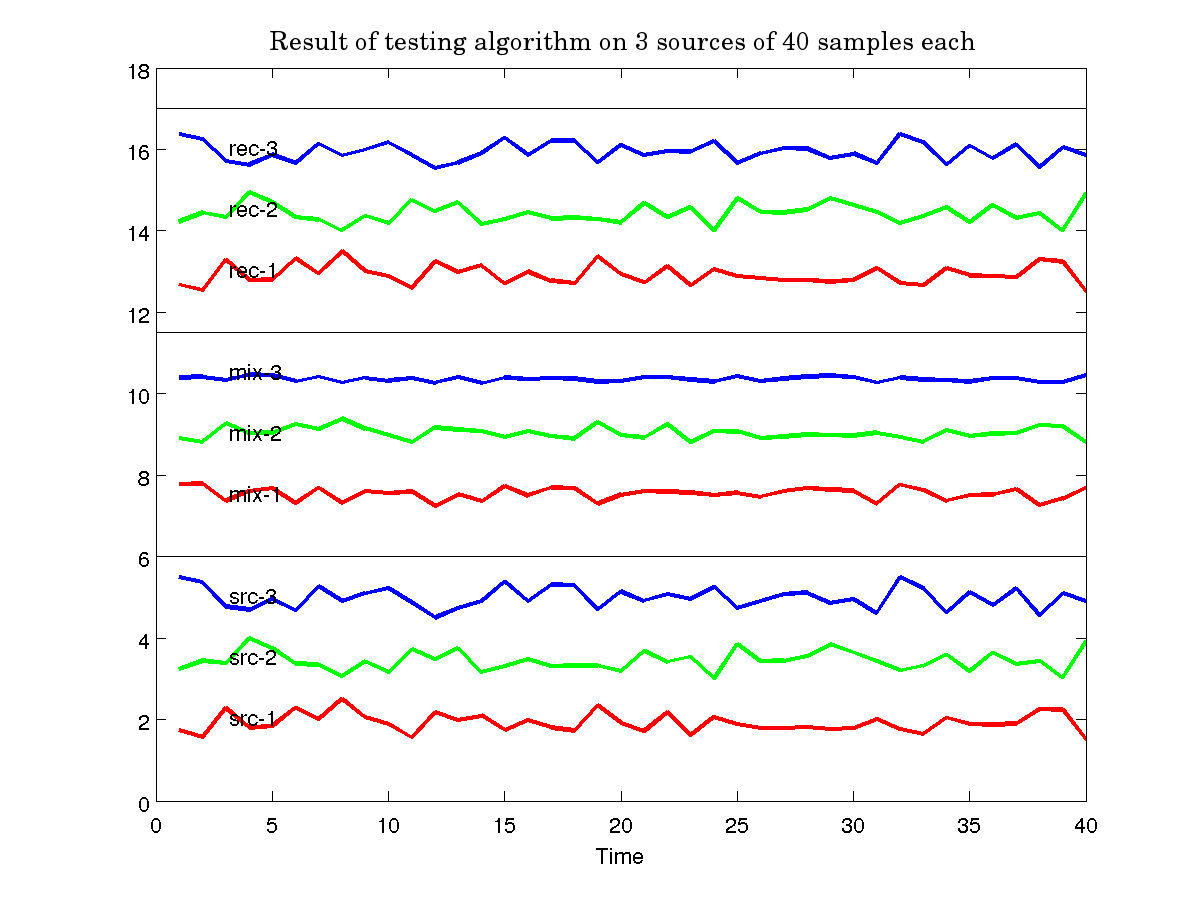
\includegraphics[width=16.0cm, height=7.0cm]{../plots/icaTestCheckImage.png}
\end{center}
\caption{Result of testing the algorithm on small 40 sample signal sources.}\label{fig:test1}
\end{figure}

\paragraph{Test Separation} 
For the test case, we set $\eta = 0.01$ and number of iterations to I$ = 1000000$. The mixing matrix contained random values (chosen uniformly at random) in the range 0 to 1. The recovered signals showed high correlation to original signals and can also be observed in Figure(\ref{fig:test1}).

\section{Results}
The original sound sources in the signal plots are marked from 1 through 5 based on the ordering in the sounds data matrix. The mapping is as follows: 1 - correponds to speaking (laws of thermodynamics). 2 corresponds to vaccum cleaner. 3 to clapping, 4 to laghter, and 5 to static noise.
\subsection{Recovering mixture of 3 sources with annealing}
The figures below show the effect of recovering a combination of 3 sources (mixed using a random mixing matrix). This experiment was performed with annealing.
\begin{figure}[hbt]
\def\tabularxcolumn#1{m{#1}}
\begin{tabularx}{\linewidth}{@{}XX@{}}
\begin{center}
   \subfloat[Recovering a mixture of 2, 3, and 4]{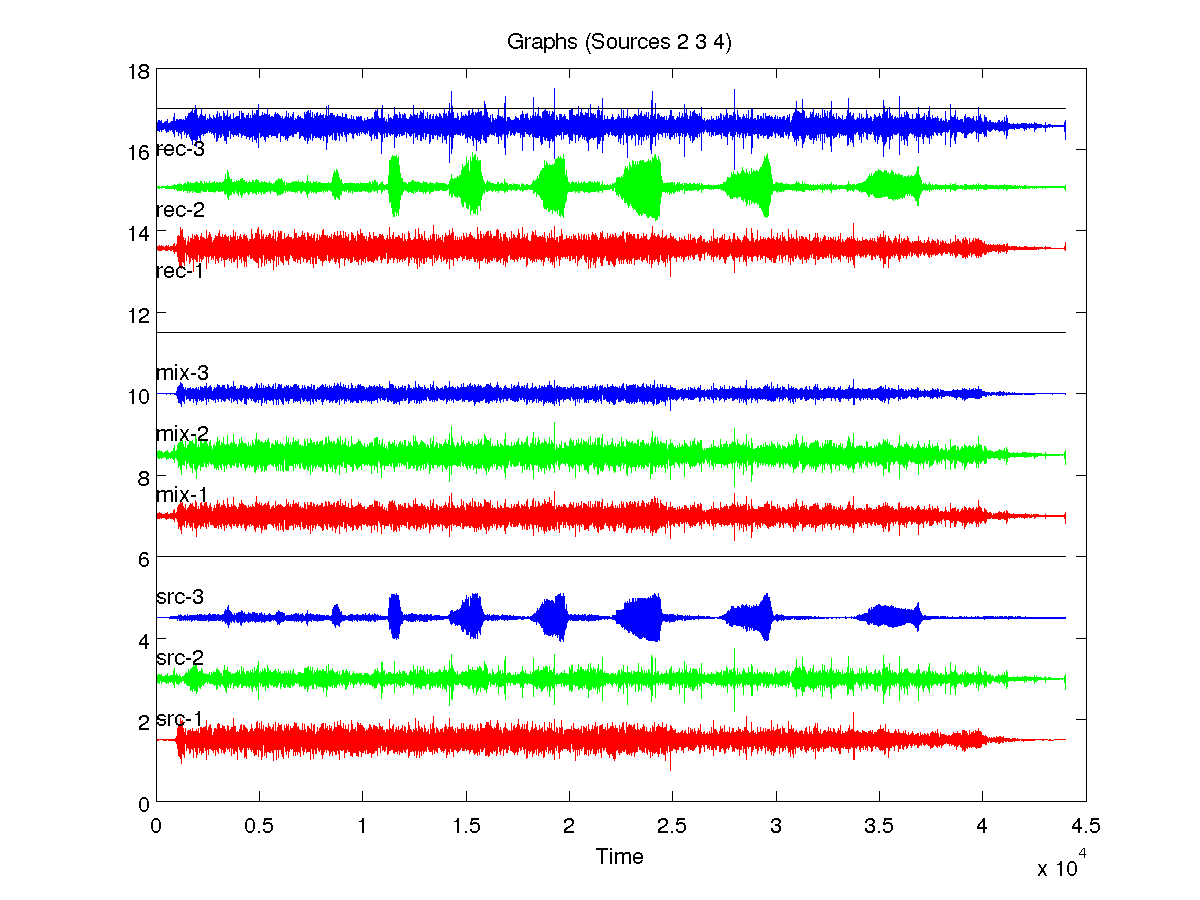
\includegraphics[width=8.5cm]{../plots/Annealrecover-srcs-234.png}}
   \subfloat[Recovering a mixture of 2, 3, and 5]{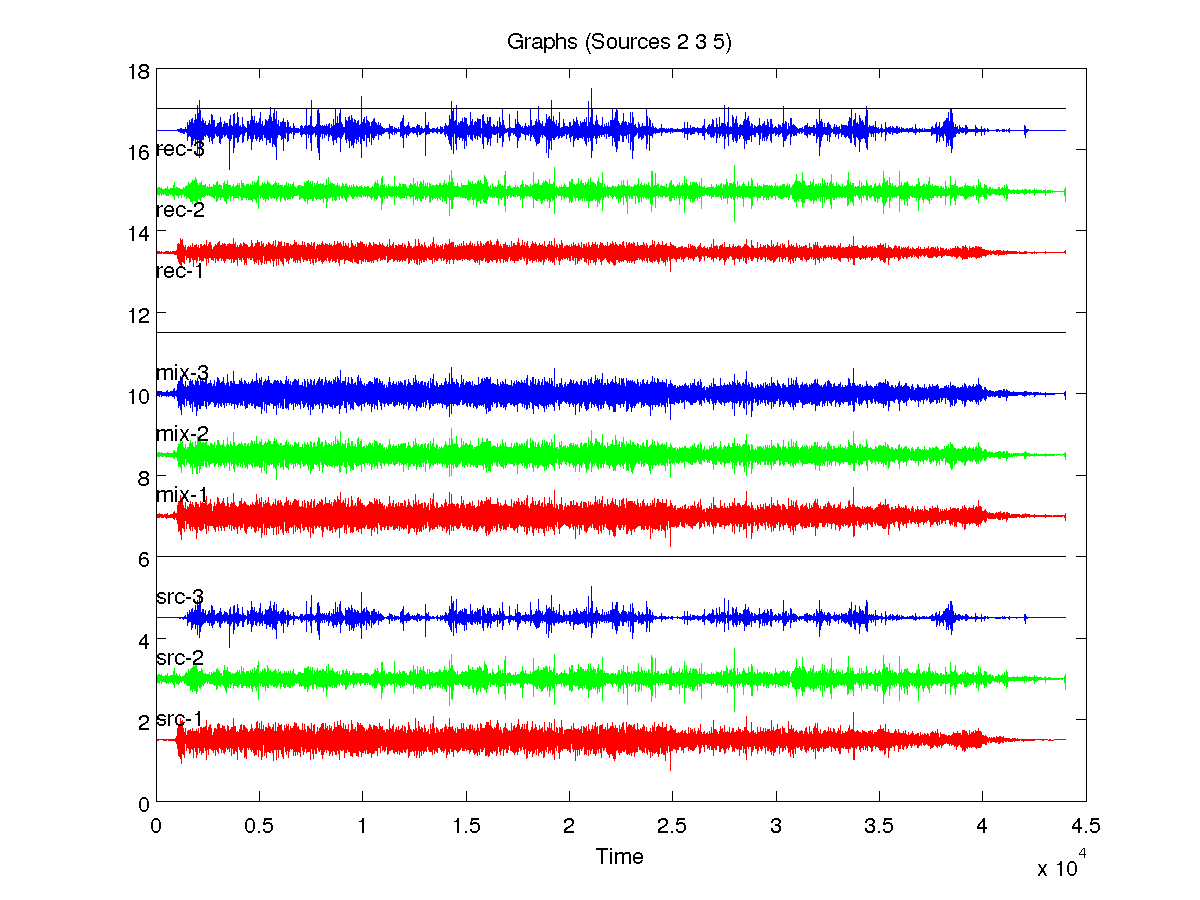
\includegraphics[width=8.5cm]{../plots/Annealrecover-srcs-235.png}}
\end{center}
\end{tabularx}
\caption{Mixture of sources 2,3, and 4; and that of 2,3, and 5, were recovered well.}\label{fig:exp2}
\end{figure}

\paragraph{Observations}
The following are some observations based on the experiment of combining three source signals and using annealing.
\begin{enumerate}
\item Annealing was extremely useful in leading the signals to converge on a good optima (atleast prevented converging on a poor local optima). Without annealing, the gradient descent algorithm usually converged to a local optimum which was not useful in separating the sources. Annealing also reduced the number of iterations required to converge (to as few as 10000).
\item Some signal combinations were better recoverable than others. It was observed that the noise of the vaccum cleaner (sound source 2), hands clapping (source 3) and laughter (source 4), were recovered fairly well. The sources corresponding to 2,3, and 5 (static noise) were also recovered reasonably well. Figure (\ref{fig:exp2}), shows the recovered signals.
\end{enumerate}

\subsection{Recovering all 5 signals}
The figures below show the effect of recovering a linear mixtures of all 5 sources (mixed using a random mixing matrix). This experiment was performed with annealing.
\begin{figure}[hbt]
%\def\tabularxcolumn#1{m{#1}}
%\begin{tabularx}{\linewidth}{@{}X@{}}
\begin{center}
%   \subfloat[Recovering a mixture of 2, 3, and 4]{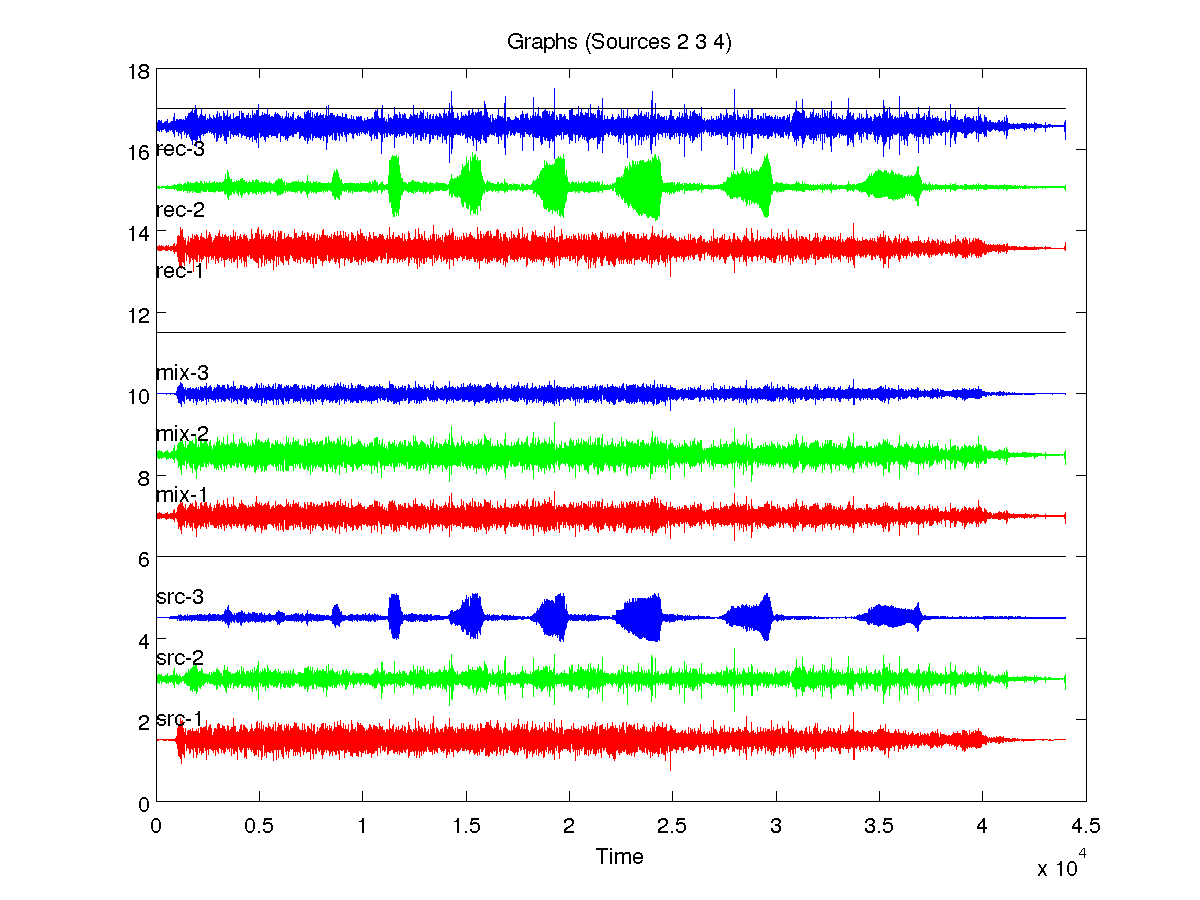
\includegraphics[width=8.5cm]{../plots/Annealrecover-srcs-234.png}}
   \subfloat[Recovering mixture of all 5 signals]{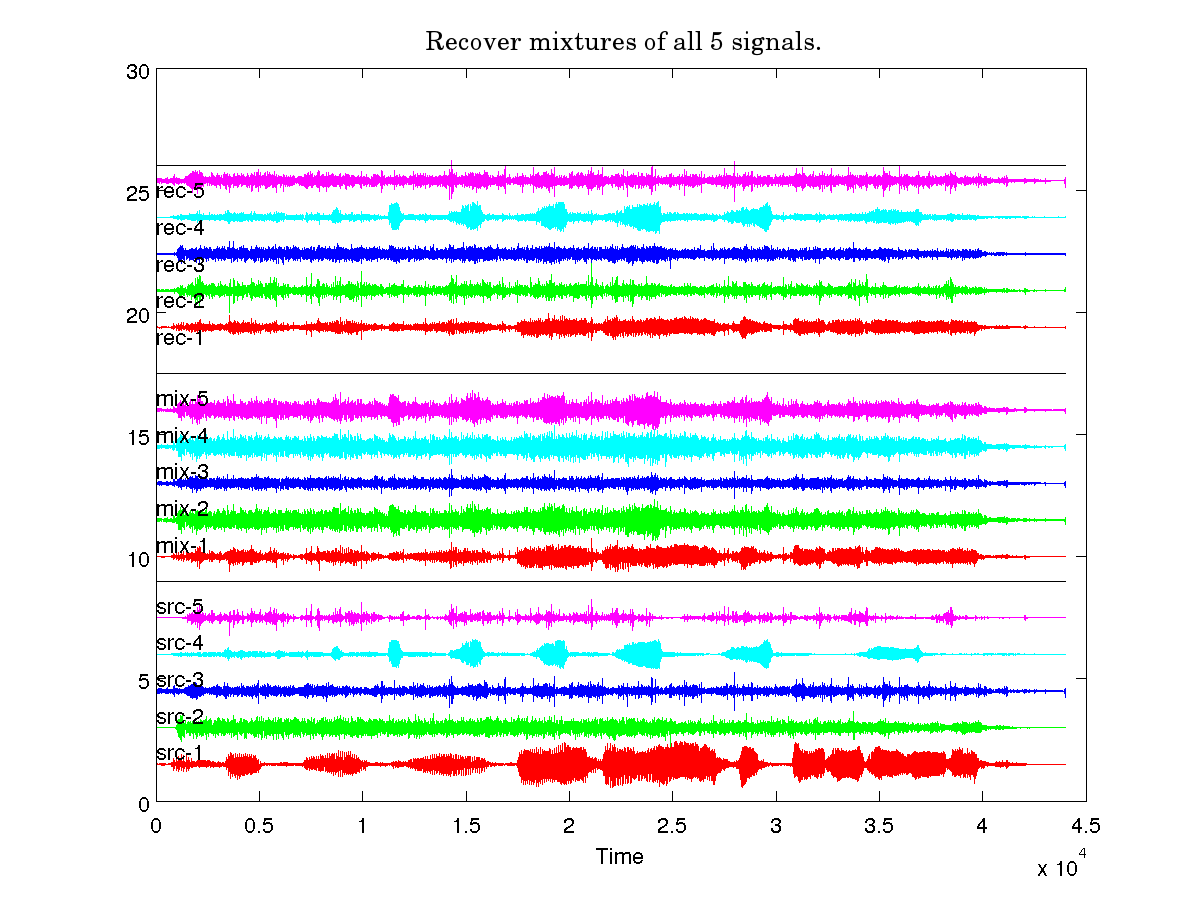
\includegraphics[width=15cm]{../plots/all5recoveredImage-10k.png}}
\end{center}
%\end{tabularx}
\caption{Mixture of sources 2,3, and 4; and that of 2,3, and 5, were recovered well.}\label{fig:exp2}
\end{figure}

\paragraph{Observations}
The following are some observations based during the experiment when recovering all 5 sources from the mixtures.
\begin{enumerate}
\item The learning rate and annealing parameters were left unchanged (compared to recovering from 3 sources). This shows that even the simeple annealing method is effective in controlling learning.
\item It was difficult to recover all the signals most of the times. Only in some of the runs all sources were recovered well. But in most of the trials, atleast a couple of sources were recovered with reasonable accuracy.
\item During the experiment it was noted that large number of iterations did not make that much of a difference.
\end{enumerate}

\subsection{Additional experiments: varying slope of sigmoid}
In addition to the regular algorithm, one can change the slope of the sigmoid to see if that affects the performance of the algorithm.We consider the new density function to be $g_i(x) = \frac{1}{(1+e^{- \beta\textbf{x}})}$ where $\beta$ is unique for each source signal. We now get the following gradient for $\beta$:
$$ \frac{\partial L}{\partial \beta_j}  = \displaystyle\sum_{i=1}^{t} x_{ji} (1 - 2g(x_{ji})) (x_{ji})^T $$
The $\beta$ values were then changed as follows:
$$ \beta_{new} = \beta_{old} + \kappa \left( \frac{\partial L}{\partial \beta_j} \right)$$

\begin{figure}[hbt]
%\def\tabularxcolumn#1{m{#1}}
%\begin{tabularx}{\linewidth}{@{}X@{}}
\begin{center}
   \subfloat[Recovering a mixture of 2, 3, and 5]{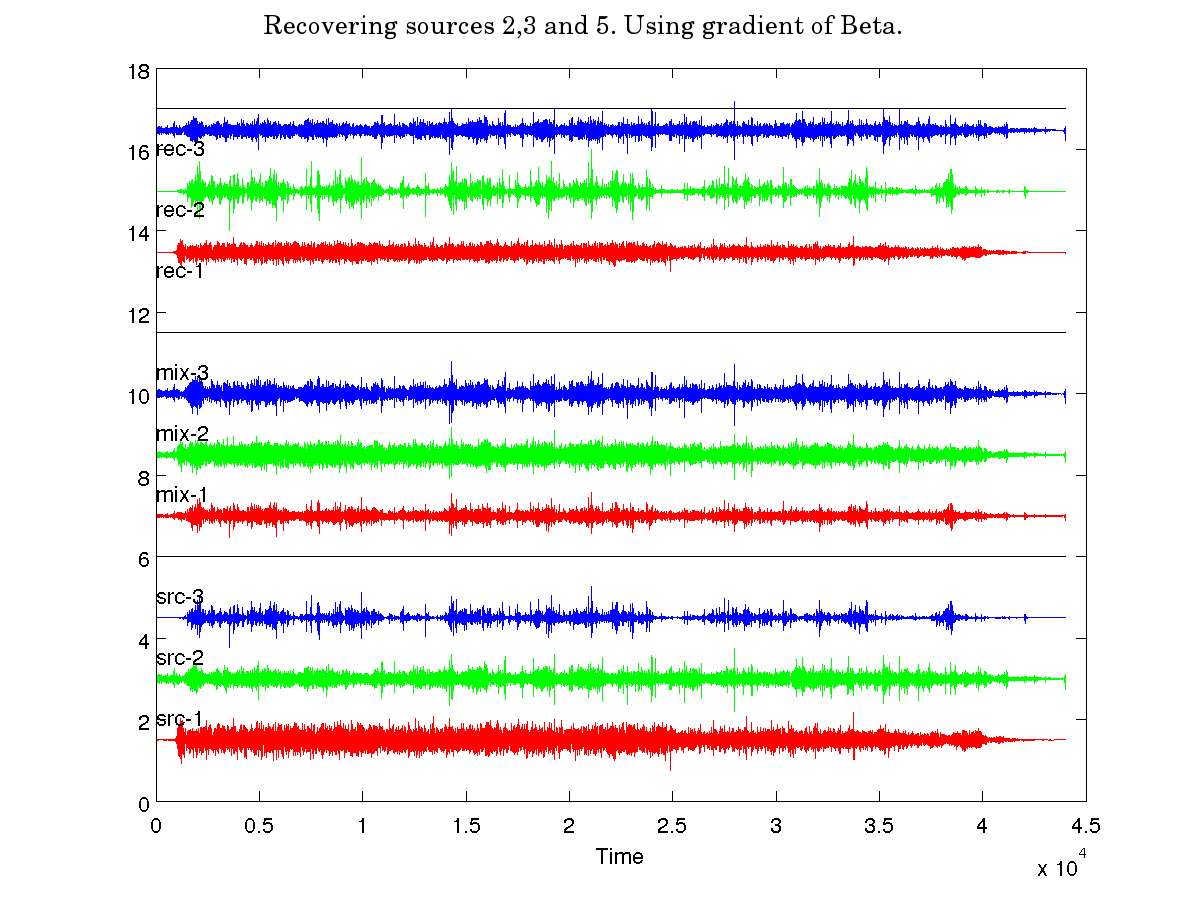
\includegraphics[width=8.5cm]{../plots/Beta-235recoveredImage-veryGood.png}}
   \subfloat[Recovering mixture of all 5 signals]{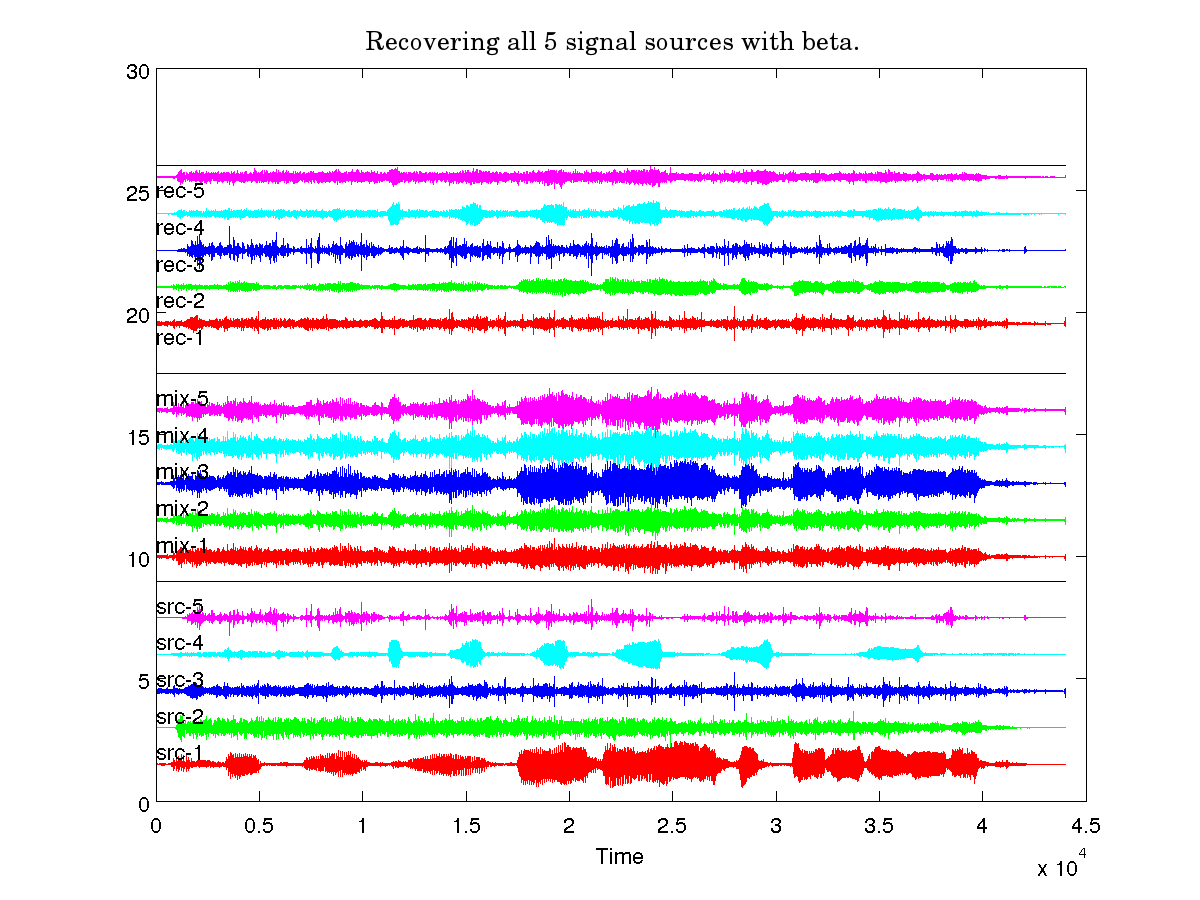
\includegraphics[width=8.5cm]{../plots/Beta-all5recoveredImage.png}}
\end{center}
%\end{tabularx}
\caption{Recovering signals by additionally varying $\beta$.}\label{fig:exp2}
\end{figure}

\paragraph{Observations}
The following are some observations based during the experiment with additional variation of $\beta$.
\begin{enumerate}
\item Setting $\kappa$ to very small values (0.0001, 0.001) did not make any change to $\beta$ values (i.e.$\beta_{new} = \beta_{old}$). The sources were recovered just as before.
\item Setting $\kappa = 0.01$ appeared reasonable. However, the actual values of $\beta_j$ (for each source were more or less very close). Here again, sources were recovered as before, but appeared slightly better (i.e running them on the same sources several times produced slightly better recovery than with out changing).
\item Setting $\kappa$ to higher values did not improve the signal recovery, infact it made it only slightly worse.
\item On increasing the number of source signals (taking all 5) considering $\beta$ did stabilize the recovery, if only marginally. i.e. On average (several trials) it appeared as though, the algorithm varying $\beta$ may have performed better.\footnote{I have not consolidated the correlation values of recovered signals across experiment trials to prove this conclusively.}
\end{enumerate}

\section{Conclusion}
This experiment proves that the ICA algorithm is surprisingly powerful and can recover a cocktail of mixed signals. However, there are several tiny caveats to note, such as, the signals need to be non-gaussian and independent, and the mixture has to be a linear mix. The additional experiment of varying $\beta$ only seemed to improve the recovery marginally. Comparing recovered signals across different trial runs should conclusively determine if variation in $\beta$ stabilizes the recovery.

\section{Appendix}
\paragraph{Comments.} 
\begin{enumerate}
\item The correlation matrices were obtained, but not presented in the report.
\item The recovered sound signals have been saved as .mat files and can be made available upon request.
\end{enumerate}

\paragraph{Code}
To see a sample run of the code, do the following on a terminal:
\begin{enumerate}
\item \tt{cd src}
\item \tt{matlab icafull.m}
\end{enumerate}
The README file explains the contents of other folders.

\end{document}
